\documentclass[11pt]{article}
\usepackage[spanish]{babel}
\usepackage[utf8]{inputenc}
\usepackage[letterpaper,margin=1in]{geometry}
\usepackage{tgheros,graphicx,fancyvrb,fancyhdr,fvextra,minted,siunitx,pgf,tikz,subcaption,float,hyperref}
\usetikzlibrary{arrows}
\renewcommand*\familydefault{\sfdefault}
\usepackage[T1]{fontenc}
\pagestyle{fancy}
\fancyfoot[C]{}
\fancyfoot[R]{\thepage}
\fancyfoot[L]{Manual GHDL + GTKWave}
\fancyhead[L,C,R]{}
\renewcommand{\footrulewidth}{0.4pt}
\renewcommand{\headrulewidth}{0pt}
\graphicspath{{img/}}
\usepackage[justification=centering]{caption}
\hypersetup{
    linkbordercolor = blue,
    colorlinks=true,       
    linkcolor=blue,         
    urlcolor=blue,
    citecolor=black,
    pdfborderstyle={S/U/W 1}
} 

\renewcommand{\labelitemi}{$\bullet$}
\thispagestyle{empty}
\newcommand{\manualtitle}[3]{
    \begingroup
        \centering
        \vspace*{2\baselineskip}
    {\Huge\textbf{#1}}\vspace*{.4\textwidth}\par
    %{\Large #2}\par\vspace*{3\baselineskip}
    
\includegraphics[width=.5\linewidth]{logo2.png}\vfill
#2\par\vspace*{\baselineskip}
        \endgroup
        \newpage
}
\begin{document}

\manualtitle{Manual GHDL + GTKWave}{Febrero 2022}


\section{Introducción} 
\setcounter{page}{1}

Este manual tiene la intención de educar al usuario
en el uso de GHDL y GTKWave como herramientas de desarrollo de
hardware utilizando VHSIC Hardware Description Language (VHDL). Se busca
que el usuario aprenda a utilizar GHDL para compilar y simular código de
VHDL, y que pueda visualizar los datos de sus simulaciones utilizando
GTKWave, haciendo uso de las diferentes herramientas de navegación para
analizar los resultados. El entorno utilizado para el desarrollo de este manual
fue de sistemas operativos basados en Linux, sin embargo, excluyendo
la instalación, las instrucciones deberán funcionar de forma uniforme
independientemente de la plataforma del usuario.

\section{Instalación} 
Para instalar los paquetes de software de GHDL
y GTKWave, se debe utilizar el gestor de paquetes de la distribución que se
tenga así como verificar si el repositorio del gestor cuenta con los
paquetes de GHDL y GTKWave. En caso contrario, se puede entrar al sitio web de
\href{http://gtkwave.sourceforge.net/}{GTKWave}
o \href{https://ghdl.github.io/ghdl/getting.html}{GHDL} para obtener binarios
pre-compilados o código fuente para compilar los programas. En el caso de Arch
Linux,Debian y Ubuntu, existen paquetes en los repositorios oficiales por lo que, en el caso 
del primero, se utiliza el gestor de paquetes \textit{pacman} como se muestra a continuación:
\begin{Verbatim}[frame=single] 
# pacman -S gtkwave ghdl 
\end{Verbatim} 
En el caso de los dos últimos, se utiliza el gestor \textit{apt} de la siguiente
forma: 
\begin{Verbatim}[frame=single] 
# apt install gtkwave ghdl
\end{Verbatim} 
En ambos casos, al momento de instalar GHDL se deberá elegir
un proveedor de herramientas para compilar el código. Existen tres opciones: 
\begin{itemize} 
    \item GCC 
    \item LLVM 
    \item mcode 
\end{itemize}

\section{Instrucciones de Uso}
Existen tres pasos para realizar una simulación con GHDL: análisis, 
elaboración y simulación, estos tres pasos se llevan a cabo
utilizando diferentes comandos de GHDL. A continuación, se describen
brevemente cada una de estas etapas, así como algunas opciones útiles.

\subsection{Análisis}

Durante esta etapa el compilador revisa cada unidad de código y la procesa
para elaborar archivos objeto (\textit{object files}) para su uso en las siguientes
etapas. En este paso se realiza el análisis semántico y sintáctico del
código. La ejecución de este paso se lleva a cabo con el siguiente
comando: 
\begin{Verbatim}[frame=single]
$ ghdl –a [opciones] archivos
\end{Verbatim}

Los argumentos de este comando consisten de una lista de archivos
(\Verb*#archivos#) cuyo orden puede ser relevante dependiendo de la 
organización del código.

\subsection{Elaboración}

En este paso se vuelve a realizar el análisis de todas las unidades de
código para generar archivos objecto que son vinculados para producir el
ejecutable que será utilizado para llevar a cabo la simulación. El comando
para este paso es el siguiente: 

\begin{Verbatim}[frame=single] 
$ ghdl –e [opciones] entidad 
\end{Verbatim}

Donde \Verb#entidad# es la entidad principal del diseño.

\subsection{Opciones para análisis y elaboración}

Las siguientes opciones aplican para los pasos de análisis y elaboración:

\begin{description} 

\item[-std=<STANDARD>] Permite elegir el estándar de
VHDL con el que se lleva a cabo la compilación. Por defecto, el estándar
es VHDL-93 (93c)

\item[-workdir=<DIR>] Especifica la dirección del directorio (DIR) donde
se encuentra el código perteneciente a la biblioteca \textit{work}. En caso de
no especificarlo, se toma por defecto la carpeta en la que se invoque el comando

\item[-p=<DIR>] Especifica la dirección del directorio (DIR) 
donde se encuentra el código perteneciente a otras bibliotecas externas que
sean requeridas

\item[-fsynopsys] Sirve para utilizar los paquetes 
\Verb*[breaklines=true,breakanywhere=true]%std_logic_arith,std_logic_signed,std_logic_unsigned,std_logic_textio%, 
que no son parte, de forma oficial, de las librerías estándar IEEE.

\end{description}

\subsection{Simulación}

Este es el último paso donde se lleva a cabo la ejecución o la simulación
del código. Este es invocado de la siguiente forma:

\begin{Verbatim}[frame=single]
$ ghdl –r [opciones] entidad [opciones de simulación]
\end{Verbatim}

Este comando acepta un primer bloque de opciones, que son las mismas
utilizadas en el análisis y la elaboración, el segundo bloque contiene
opciones específicas para la simulación que son descritas más adelante.
Finalmente, la entidad que se pasa como argumento es aquella que se busca
simular.

\subsubsection{Opciones}

Algunas opciones útiles para la simulación son descritas a continuación.

\begin{description} 
\item[-{}-disp-time] Muestra el tiempo y los ciclos delta 
    (\textit{delta cycles}) que lleva la simulación mientras se ejecuta

\item[-{}-stop-delta=<N>] Detiene la simulación después de \textit{N} ciclos
    delta. El valor por defecto para esta opción es de 5000 ciclos

\item[-{}-stop-time=<T>] Detiene la simulación después de un intervalo de
    tiempo \textit{T}, donde \textit{T} esta expresado en unidades de una variable 
    \textit{time} de VHDL. Cabe resaltar que este tiempo es relativo a la simulación 
    y no al reloj interno del diseño.

\item[-{}-wave=<FILE>] Guardar las salidas de las señales en un archivo
    con dirección \textit{FILE} en formato GHDL Waveform (GHW)

\item[-{}-vcd=<FILE>/-vcdgz=<FILE>] Guardar las salidas de las señales en
    un archivo con dirección FILE con formato VCD. La opción \textit{-vcdgz} tiene
    la característica adicional que comprime los datos de las señales con gzip. 
\end{description} 

El uso de GTKWave para visualizar las simulaciones se describe utilizando los
siguientes ejemplos.

\section{Ejemplo 1: Simulación simple}

En este ejemplo se lleva a cabo la simulación de una arquitectura que
describe una señal de reloj mediante un proceso. Este diseño no tiene
ninguna entrada y solo una salida (\textit{CLK}). A continuación, se muestra el
código de esta entidad:

\inputminted[frame=single, framesep=4mm, label=\fbox{clock.vhd},
labelposition=bottomline]{vhdl}{src/clock.vhd}

El paso de análisis se lleva a cabo con el siguiente comando:

\begin{Verbatim}[frame=single]
$ ghdl -a clock.vhd
\end{Verbatim}

Posteriormente, la elaboración se lleva a cabo con el siguiente comando:

\begin{Verbatim}[frame=single]
$ ghdl -e clock
\end{Verbatim}

Es importante resaltar que para este paso, el argumento del comando es el
nombre de la entidad (\textit{Clock}) y no el nombre del archivo, además, se tiene que
considerar que VHDL no es un lenguaje que distinga entre letras mayúsculas y
minúsculas, por lo que tampoco importa que el nombre de la entidad sea idéntico
al del argumento del comando, al menos en este aspecto.

Finalmente, para realizar la simulación se debe ejecutar el siguiente comando:

\begin{Verbatim}[frame=single]
$ ghdl -r clock --wave=clock_sim.ghw
\end{Verbatim}

En este caso, el archivo de salida para las señales es \textit{clock\_sim.ghw}.
Con estas opciones, la operación de simulación deberá ser detenida manualmente,
utilizando CTRL+C. Otra forma de realizar esta operación es utilizando la
opción \textit{-{}-stop-time} como se muestra a continuación:

\begin{Verbatim}[frame=single]
$ ghdl -r clock --wave=clock_sim.ghw --stop-time=5us
\end{Verbatim}

De esta forma, la simulación termina de forma automática, después de
5\unit{\micro\second}.

Para analizar la simulación con GTKWave, se puede invocar al programa desde la
consola utilizando como argumento, el archivo de salida con las señales de la
simulación (en este caso \Verb*#clock_sim.gwh#), como se muestra en el siguiente
comando:

\begin{Verbatim}[frame=single]
$ gtkwave clock_sim.ghw
\end{Verbatim}

O bien, arrancar directamente el programa y abrir desde ahí el archivo de las
señale con la opción \textit{File} > \textit{Open New Tab}. Una vez que GTKView ha 
arrancado, se muestra la pantalla principal (Figura \ref{fig:gtkwave-1}).

\begin{figure}[H]
\centering
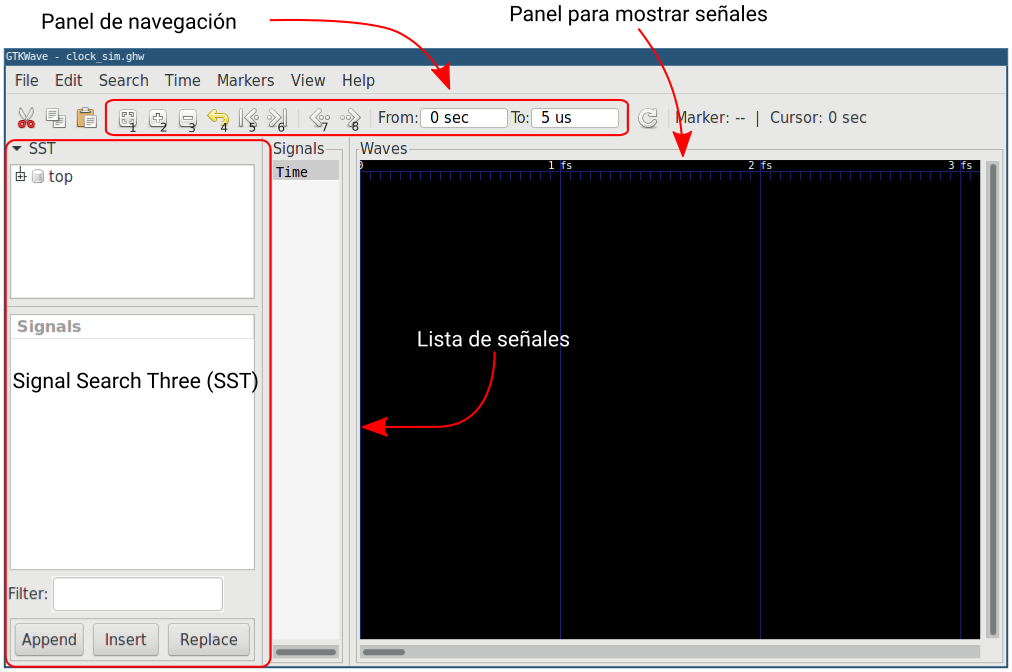
\includegraphics[width=.75\linewidth]{gtkwave-menu.png}
\caption{Pantalla principal de GTKWave}
\label{fig:gtkwave-1}
\end{figure}

Algunos de sus elementos más importantes se describen en seguida.

\begin{description}

\item[Signal Search Tree (SST)] Es un menú acomodado de forma jerárquica de acuerdo
    con el diseño de la entidad. Al seleccionar un elemento del menú, sus señales
    aparecerán en el apartado inferior con la etiqueta \textit{Signals}. Este panel puede
    ser usado para arrastrar las señales que se quieran visualizar, arrastrándolas
    hacía la lista que se encuentra la derecha (\textit{Signals}). Otra forma de hacer esto
    es dar clic derecho en la entidad o la señal y seleccionar la opción \textit{Recurse
    Import} y elegir si se quiere agregar al final (\textit{append}), al
    inicio (\textit{insert}) o reemplazarla(\textit{replace}) en la lista de señales de la derecha.

\item[Signals] Es una lista que contiene todas las señales que se muestran, así como
    su valor en el instante en que se encuentre parado el cursor. Al hacer clic
    derecho en los elementos contenidos en esta lista se pueden hacer ajustes para
    la visualización de las señales como cambiar el color de la onda o seleccionar
    la representación con la que muestran sus valores (binario, decimal, hexadecimal, etc.)

\item[Waves] Es el panel donde se muestran los datos de la simulación en forma de
    ondas. Dentro de este espacio se puede utilizar la funcionalidad de los
    cursores primario y secundario, ajustando cada uno con el clic izquierdo y el
    clic intermedio del ratón, respectivamente, para analizar las señales.

\item[Panel de navegación] Este panel contiene botones para moverse a lo largo de las
    señales de la simulación. El primer botón (1) sirve para ajustar la escala de la
    señal al tamaño de la ventana, mientras que los siguientes dos sirven para
    aumentar(2) o reducir(3) la escala, el siguiente botón(4) sirve para deshacer la última
    modificación a la escala que se haya hecho mediante estos botones. Los
    siguientes dos botones sirven para recorrer el área que se muestra de las
    señales, al final (5) o al inicio(6) de la simulación. Finalmente, los últimos dos
    botones sirven para moverse entre el flanco anterior (7) o el siguiente(8) de cada
    señal. Los campos \textit{From} y \textit{To} sirven para delimitar el segmento de
    tiempo de la simulación que es mostrado.
\end{description}

Una vez que se ha abierto el archivo, se tienen que elegir las señales que se
quieren mostrar, para este ejemplo se agregan las señales de toda la
entidad desde el SST (Figura \ref{fig:gtkwave-2}).

\begin{figure}[H]
\begin{subfigure}[c]{.5\linewidth}
    \centering
    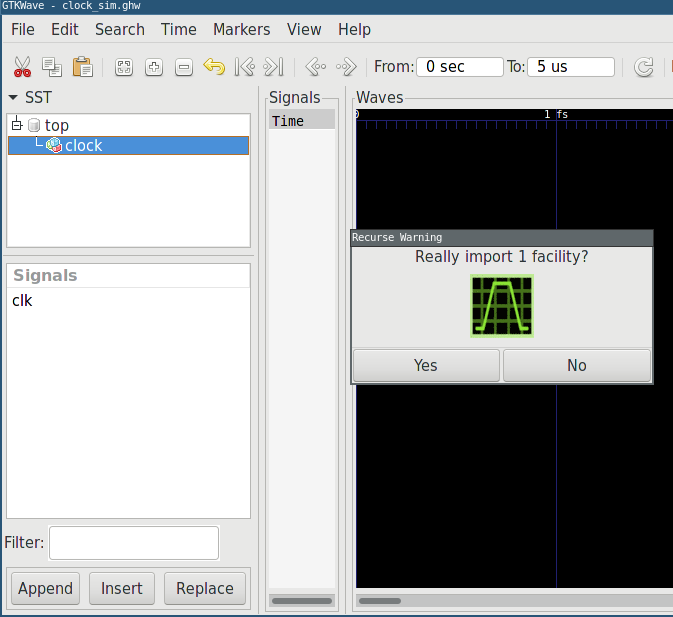
\includegraphics[height=.62\textwidth]{gtkwave2a.png}
    \caption{Agregando señales}
    \label{fig:gtkwave-2}
\end{subfigure}
\begin{subfigure}[c]{.5\linewidth}
    \centering
    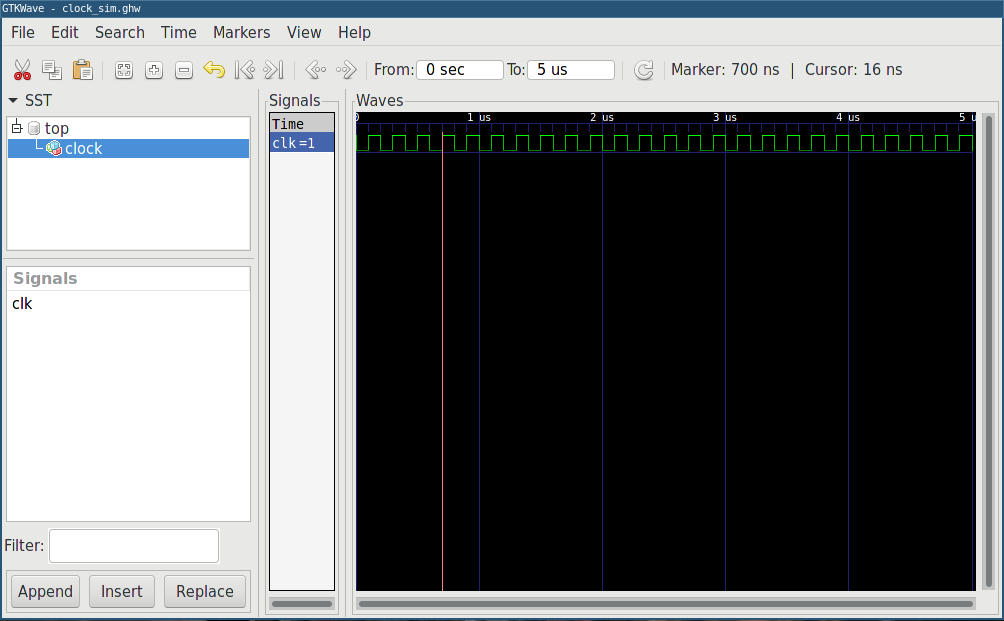
\includegraphics[height=.62\textwidth]{gtkwave3.png}
    \caption{Simulación de la entidad}
    \label{fig:gtkwave-3}
\end{subfigure}
\caption{Simulación de la entidad Clock}
\end{figure}

Finalmente, en la Figura \ref{fig:gtkwave-3} podemos observar la señal del 
reloj de 5 \unit{\kilo\hertz} (T = 200 \unit{\nano\second}), simulada por 5
\unit{\micro\second}.

\section{Ejemplo 2: Simulación con paquetes}\label{sim-2}

En un diseño más complejo es de utilidad dividir la funcionalidad en diferentes
paquetes encargados de realizar tareas específicas, dentro de estos paquetes se
pueden definir constantes, componentes y funciones. Para el siguiente ejemplo
se simulará una Unidad Aritmética-Lógica (ALU) diseñada para trabajar con
\textit{N} bits, esta unidad está diseñada a partir de un componente básico que 
es la ALU de 1 bit, que a su vez depende del componente sumador de 1 bit (el
código de cada entidad se encuentra en el apéndice \nameref{appendix-a}). La
jerarquía de componentes se muestra en la Figura \ref{fig:alu-jerarquia}:

\begin{figure}[H]
\centering
\begin{tikzpicture}
\node (tb)      at (1,3) {Testbench: Archivo de pruebas (Testbench.vhd)};
\node (alun)    at (2,2) {ALUNBits: ALU de N bits (ALUNbits.vhd)};
\node (alu1)    at (3,1) {ALUBit: ALU de 1 bit (ALUBit.vhd)};
\node (sum1)    at (4,0) {sumaBit: Sumador de 1 bit (sumaBit.vhd)};
\draw (tb.west)     -- ++(-3mm, 0mm) -- ++ (0mm,-1) -- (alun.west);
\draw (alun.west)   -- ++(-3mm, 0mm) -- ++ (0mm,-1) -- (alu1.west);
\draw (alu1.west)   -- ++(-3mm, 0mm) -- ++ (0mm,-1) -- (sum1.west);
\end{tikzpicture}
\caption{Jerarquía de componentes para la ALU de \textit{N} bits}
\label{fig:alu-jerarquia}
\end{figure}

Esta jerarquía es importante al momento invocar los comandos de análisis,
elaboración y simulación. Dado que las definiciones del sumador de un bit y la
ALU de un bit se encuentran dentro del paquete \textit{ALUPackage}, este se tiene que
colocar al principio de la lista, seguido de los archivos que describen estos
componentes (ALU y sumador), para que al momento que se analice la entidad
\textit{ALUNBits}, el compilador ya tenga registrados esos componentes y lo mismo suceda
al analizar el testbench. La invocación del comando para analizar es la siguiente:

\begin{Verbatim}[frame=single] 
$ ghdl -a ALUPackage.vhd sumaBit.vhd ALUBit.vhd ALUNbits.vhd Testbench.vhd 
\end{Verbatim}

La entidad que es pasada como argumento debe de ser la de mayor jerarquía por
lo que utilizamos \textit{ALUNBits} como se muestra a continuación:

\begin{Verbatim}[frame=single]
$ ghdl -e ALUNbits
\end{Verbatim}

Una vez que se ha elaborado la entidad que va a ser simulada, se elabora el
testbench:

\begin{Verbatim}[frame=single]
$ ghdl -e Testbench.
\end{Verbatim}

Finalmente, se invoca al comando de simulación con la opción \textit{-{}-wave} para
exportar los datos de las señales a un archivo \textit{GHW}. Como el proceso de este
testbench acaba con una instrucción \textit{wait} con tiempo indeterminado, la simulación
sale de la ejecución de forma automática, por lo que no se requiere la opción
\textit{-{}-stop-time} ni la salida manual del programa.

\begin{Verbatim}[frame=single]
$ ghdl -r testbench --wave=alun_tb.ghw
\end{Verbatim}

Posteriormente abrimos el archivo \textit{alun\_tb.ghw} con GTKWave, al
expandir el árbol del SST podemos observar que aparecen las señales del
testbench así como todas las señales internas de la entidad \textit{ALUNbits}
(Figura \ref{fig:gtkwave-4}).
Elegimos una mezcla de señales internas de la entidad \textit{alu} como
las banderas \textit{overflow} (OV), cero(Z), \textit{carry}(C), negativo (N),
los buses de las dos entradas \textit{a} y \textit{b} y la salida de datos
\textit{s}. En la Figura \ref{fig:gtkwave-5} se pueden ver todas estas señales
ya agregadas a la lista de señales.
Después de haber agregado estas señales, podemos utilizar  las opciones del
menú de cada señal (Figura \ref{fig:gtkwave-6}) para cambiar la 
representación en la que se muestran los valores de las señales por algo más útil como 
decimal con signo, que nos permite apreciar los resultados de operaciones aritméticas. 
Como se puede ver en la Figura \ref{fig:gtkwave-7}, en los primeros 10
\unit{\nano\second} se hace una suma, mientras que en los siguientes 10
\unit{\nano\second} se hace la resta. 

\begin{figure}[H]
    \centering
    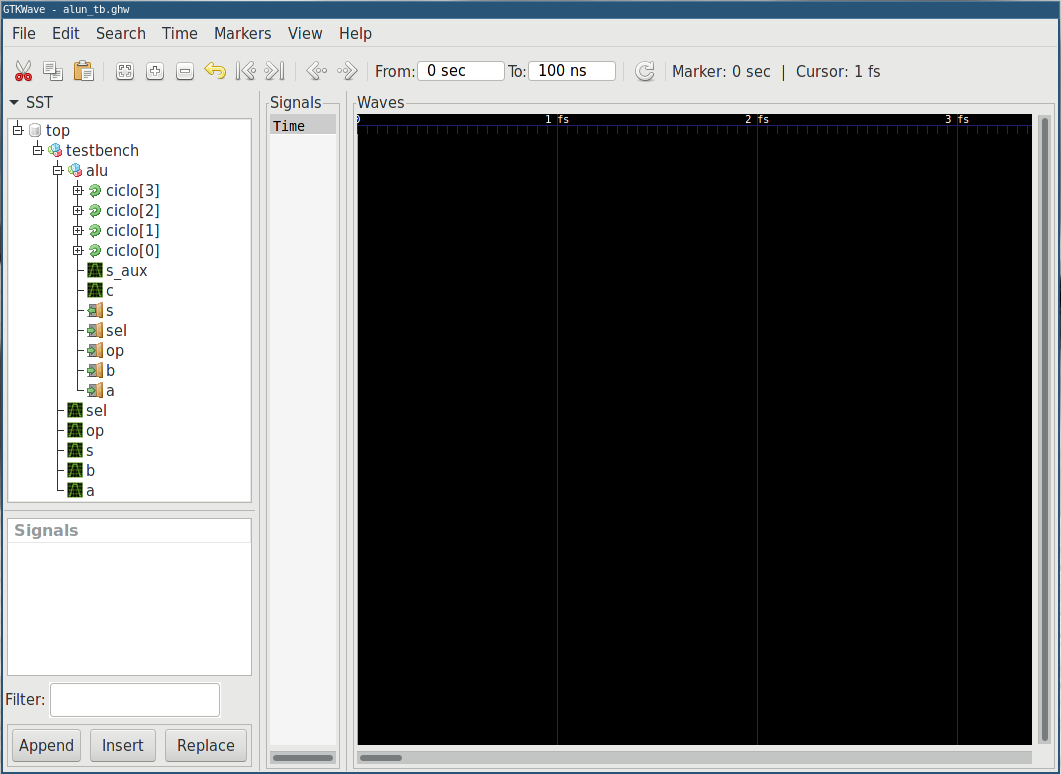
\includegraphics[width=.65\linewidth]{gtkwave4.png}
    \caption{GTKWave con las señales cargadas desde el archivo
    \textit{alun\_tb.ghw} mostradas en el panel del SST}
    \label{fig:gtkwave-4}
\end{figure}

\begin{figure}[H]
    \centering
    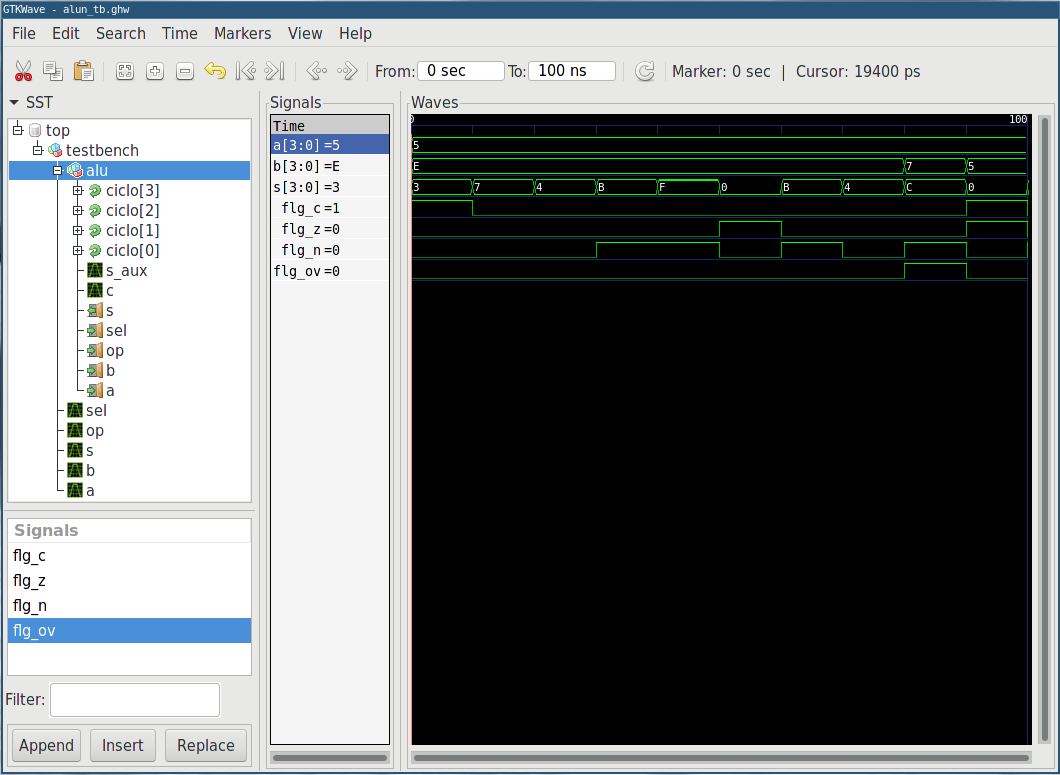
\includegraphics[width=.75\linewidth]{gtkwave5.png}
    \caption{Señales seleccionadas de la ALU en el panel de visualización de señales}
    \label{fig:gtkwave-5}
\end{figure}

\begin{figure}[H]
    \centering
    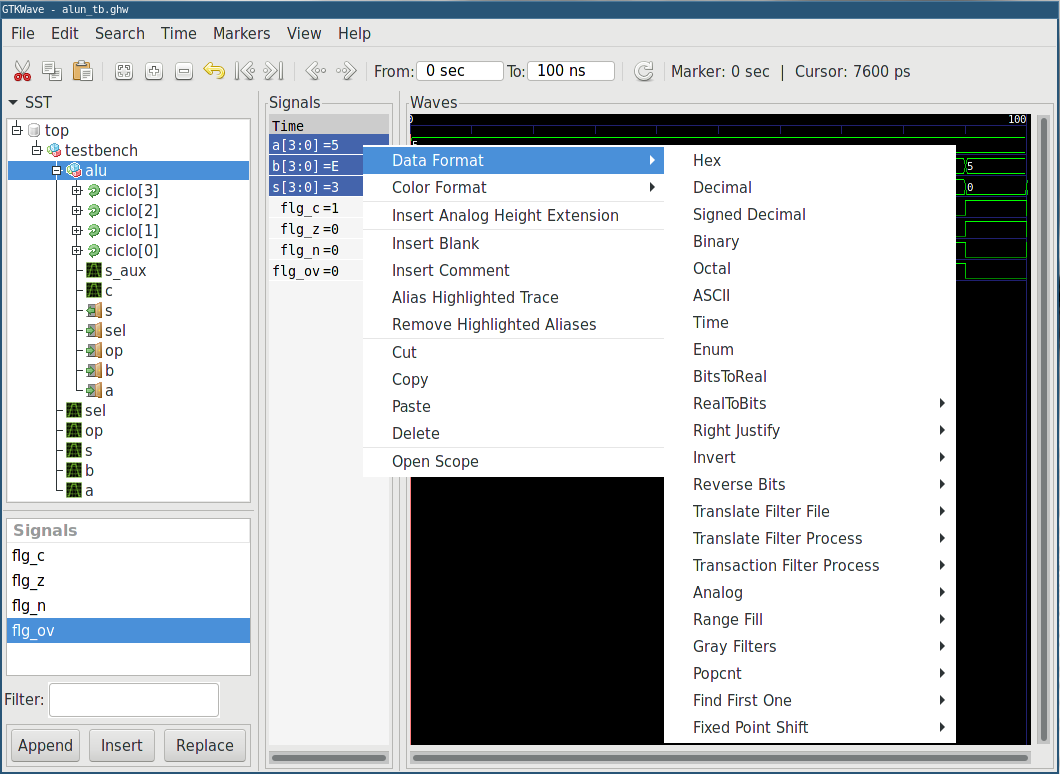
\includegraphics[width=.75\linewidth]{gtkwave6.png}
    \caption{Menú para cambiar la representación de los valores de las señales, se pueden
    ver las diferentes opciones como binario, decimal, hexadecimal, octal, etc.
    Se elige la representación}
    \label{fig:gtkwave-6}
\end{figure}

\begin{figure}[H]
    \centering
    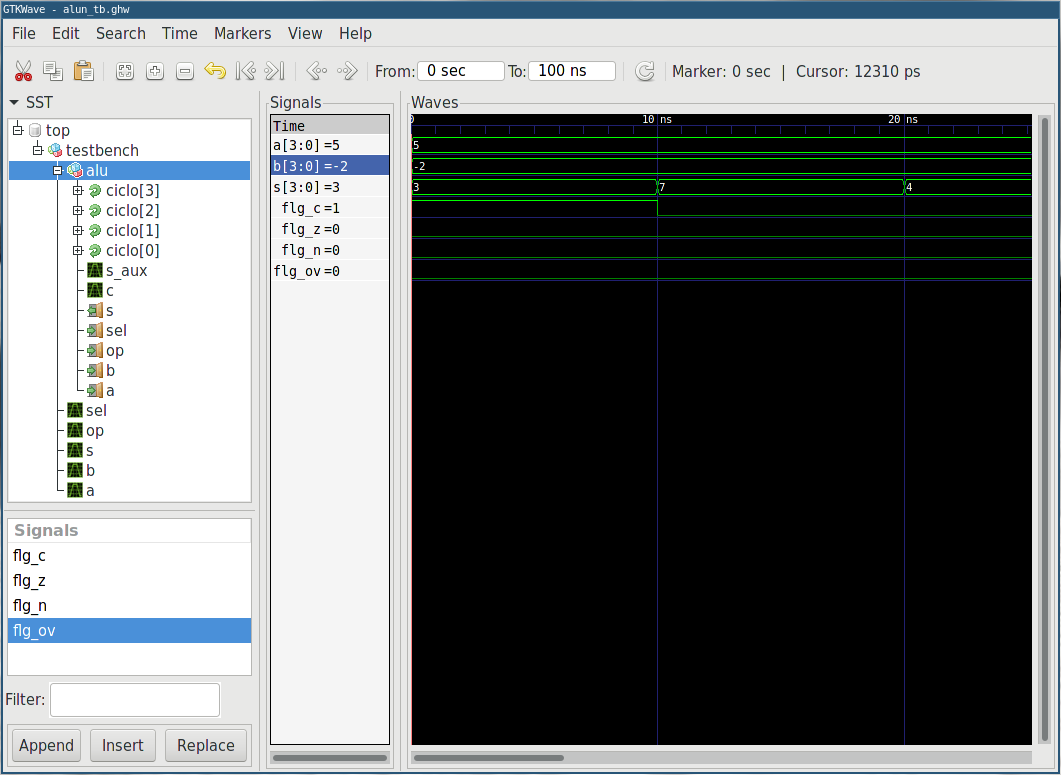
\includegraphics[width=.75\linewidth]{gtkwave7.png}
    \caption{Primeros 20 \unit{\nano\second} de la simulación donde se hace una
    suma ($s = a+b$ donde $a = 5$,$b = -2$) y una resta ($s = a-b$)}
    \label{fig:gtkwave-7}
\end{figure}

\section{Lectura adicional}

Hasta ahora hemos explorado las funciones más básicas de GHDL y GTKWave, 
sin embargo, existen otras funciones que también pueden ser útiles para el 
usuario en el desarrollo de diseños digitales, todas estas funciones se 
encuentran documentadas en el \href{http://gtkwave.sourceforge.net/gtkwave.pdf}{manual} 
de GTKWave y la \href{https://ghdl.github.io/ghdl/index.html}{documentación} de
GHDL, cuya lectura es recomendada.

\appendix

\newpage
\section{Código de pruebas} \label{appendix-a}

\subsection{Sumador de 1 bit (\textit{sumaBit.vhd})}
\inputminted[frame=lines, framesep=4mm]{vhdl}{src/sumaBit.vhd}

\subsection{ALU de 1 bit (\textit{ALUBit.vhd})}
\inputminted[frame=lines, framesep=4mm]{vhdl}{src/ALUBit.vhd}

\subsection{ALU de N bits (\textit{ALUNbits.vhd})}
\inputminted[frame=lines, framesep=4mm]{vhdl}{src/ALUNbits.vhd}

\subsection{Paquete con definiciones para la ALU (\textit{ALUPackage.vhd})}
\inputminted[frame=lines, framesep=4mm]{vhdl}{src/ALUPackage.vhd}

\subsection{Testbench (\textit{Testbench.vhd})}
\inputminted[frame=lines, framesep=4mm]{vhdl}{src/Testbench.vhd}

\end{document}
